\documentclass[titlepage, 11pt]{article}
\usepackage{fixltx2e}
\usepackage{titlesec}

\titleformat*{\section}{\LARGE\bfseries}
\titleformat*{\subsection}{\large\bfseries}


\setlength{\oddsidemargin}{0.0in}
\setlength{\evensidemargin}{0.0in}
\setlength{\topmargin}{-0.25in}
\setlength{\headheight}{0in}
\setlength{\headsep}{0in}
\setlength{\textwidth}{6.5in}
\setlength{\textheight}{9.25in}
\setlength{\parindent}{0in}
\setlength{\parskip}{2mm}
\usepackage{listings, caption, color, xcolor, graphicx}
\pagestyle{plain}

\definecolor{gray}{rgb}{0.5,0.5,0.5}
\lstset{
basicstyle=\footnotesize\ttfamily,
breaklines=true,
captionpos=t,
numbers=left,
numbersep=5pt,
numberstyle=\tiny\color{gray},
tabsize=2,
title=\lstname,
language=C++,
keywordstyle=\bfseries\color{green!30!black},
commentstyle=\itshape\color{gray},
identifierstyle=\color{blue!40!black}
}

\captionsetup{labelformat=empty}

\title{\Huge ECS 158 Final Report: \\\LARGE combn() in Snow, OpenMP, and CUDA}
\date{}
\author{\huge Stefan Peterson\\\huge Bijan Agahi \\\huge Arjun Bharadwaj}

\begin{document}
\maketitle
\begin{abstract}
Parallel architectures are becoming increasingly prevalent in the modern world and as such have spawned multiple frameworks to assist with parallel programming, but these frameworks vary greatly in their implementation and performance. This paper takes a close look at three frameworks: R-Snow, OpenMP and CUDA. We took on the task of re-writing the combn() function found in R using each of these frameworks. We measure run times of these tests at different sizes and with varying inputs and levels of difficulty. In the end, we point out the strengths and weaknesses of each language as well as note on features which we, as programmers, find particularly useful or troublesome.
\end{abstract}
\tableofcontents
\newpage
\section{Introduction}
With the relatively recent introduction of widely available multi-processor CPUs in household computers, parallel programming has become a hot topic in the world of computer science. In particular, the graphics and games industry has driven the multithreaded programming style to the forefront of everyone's attention. Through the process of splitting up tasks and distributing those tasks to individual cores on the CPU or GPU, parallel processing in most cases can provide vast improvements in both performance and efficiency. OpenMP, R-Snow, and CUDA are three such parallel languages, and this paper aims to compare and contrast the strengths, weaknesses, and performance of each language.

\subsection{Setup for Benchmarks}
All tests for the purposes of this paper were run on Tetraat University of California, Davis. This computer consists of a 64-bit 8-core processor with 16 GB or RAM and an Intel Core i7-2600K CPU with a clock speed of 3.4 GHz and a cache size of 8192 KB. The machine was running release 19 of the linux distribution Fedora.

\section{combn() in R-Snow}

\subsection{combn() in R-Snow: Strategy}

\subsection{combn() in R-Snow: Implementation}


\subsection{combn() in R-Snow: Data}

\subsection{combn() in R-Snow: Analysis}

\section{combn() in OpenMP}
\subsection{Strategy}
For the OpenMP version of the combinations function, we decided to parallelize by dedicating each thread to a subsection of the problem 

\subsection{Implementation}

\begin{center}\textcolor{black!50}{All the references to code will be references to Appendix: A.1}\\ \end{center}
We decided to take a recursive approach to the implementation of the combinations function in C++. The core functionality of the program can be found on lines 23-33 in the method findCombs. This method takes in as its parameters 2 integers, a vector, and a 2d vector. Upon the first call of findCombs() the vector combination will already have been initialized to contain the first value in the combination (i.e. if we assume we are looking for the combination [1,2,3] the vector will be initialized to contain [1] and this is done on line 71 in the combn() function. From there the recursive algorithm will add the next number (i.e. combinations will now contain [1,2]) and then will call findCombs() recursively until the base case is met upon which the vector combination is pushed on to the 2D vector. When the recursion is done and the 2D vector contains all its possible combinations, the function vectorToArray() is called and the 2D vector is parsed and its values are added to the appropriate region of the global array. 


\subsection{Data}
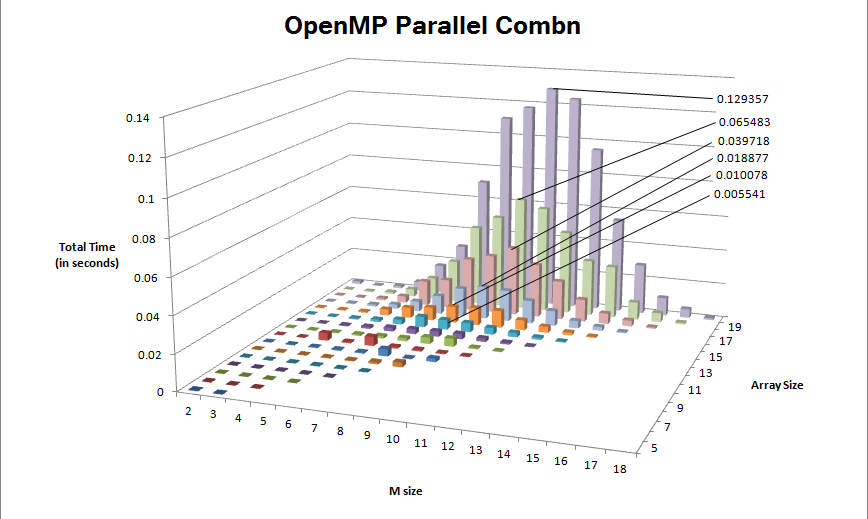
\includegraphics[scale = 0.5]{3D-OMP.png} \\

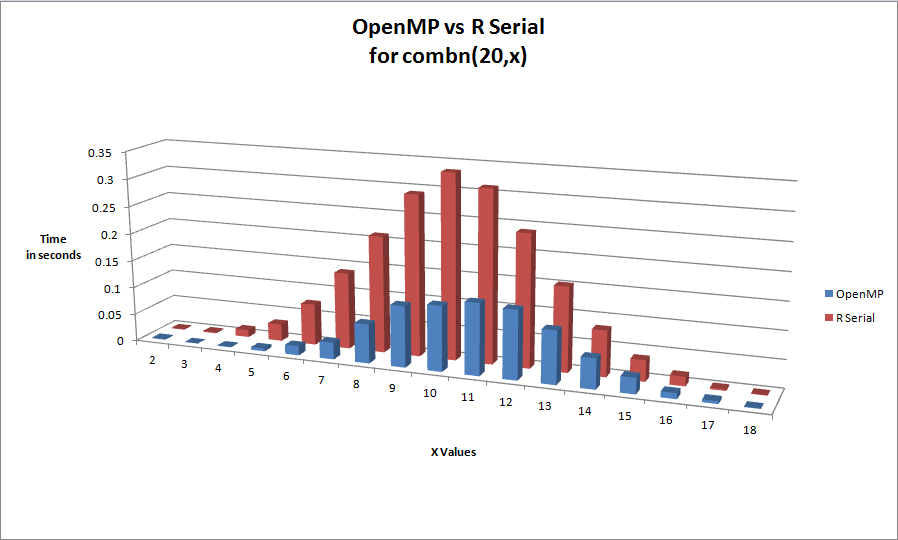
\includegraphics[scale = 0.5]{OMPvsR.png}

\subsection{Analysis}

\section{combn() in Thrust}

\subsection{combn() in Thrust: Strategy}

\subsection{combn() in Thrust: Implementation}

\subsection{combn() in Thrust: Data}

\subsection{combn() in Thrust: Analysis}




\section{Research Papers}

\subsection{Authors --- Position}

\subsubsection{Description}

\subsubsection{Analysis}







\section{Conclusion}
stuff here




\section{Bibliography}


\pagebreak
\appendix
\section{Appendix: Code}
\subsection{combn() --- OpenMP implementation}
\lstinputlisting[language=C++, caption=combnOpenMP.cpp]{combnOpenMP.cpp}
This is a recursive implementation of the combinations function. Here we used \verb; #pragma omp parallel for schedule(dynamic); on line 67 to help load balance the parallelization of the threading.  \\
\subsection{combn() --- Thrust implementation}
\lstinputlisting[language=C++, caption=combnThrust.cilk]{combn.cu}
This code is directly translate from the OpenMP version above, using the same algorithm. We have various Cilk++ equivalents of OpenMP, including: the 
\\


There are also a variety of files specific for testing purposes included in the submitted .tar file.

\newpage
\section{Appendix: Member Contributions}

\textbf{Stefan Peterson}
\begin{itemize}
	\item \LaTeX{} Formatting, editing
	\item OpenMP implementation
	\item Abstract
	\item Introduction
	\item Research paper summarization/analysis
	\item Conclusion
	\item Data analysis writeup
	\item Relevant research
\end{itemize}

\textbf{Bijan Agahi}
\begin{itemize}
	\item R-Snow implementation
	\item Experiment data collection
	\item Test scripting
	\item Graphing in R, tabling
	\item Relevant research
\end{itemize}

\textbf{Arjun Bharadwaj}
\begin{itemize}
	\item Thrust implementation
	\item Relevant research
\end{itemize}

\end{document}